\documentclass[tikz]{standalone}

\begin{document}

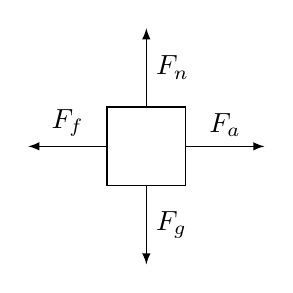
\begin{tikzpicture}
    % Draw the box
    \draw (0,0) rectangle ++(1,1);
    
    % Draw the forces:
    % Gravity
    \draw[>=latex, ->] (0.5,0) -- ++(0,-1) node[midway, right] {$F_g$};
    % Normal
    \draw[>=latex, ->] (0.5,1) -- ++(0,1) node[midway, right] {$F_n$};
    % Applied
    \draw[>=latex, ->] (1,0.5) -- ++(1,0) node[midway, above] {$F_a$};
    % Friction
    \draw[>=latex, ->] (0,0.5) -- ++(-1,0) node[midway, above] {$F_f$};
\end{tikzpicture}

\end{document}